\section{Management Summary}
\subsection*{Ausgangslage}
Open Street Map, eine online Kartenanwendung wie Google Maps, bietet seinen Benutzern eine Fussgängernavigation an. Der Nutzer wird dabei entlang von Strassen und Wegen zu seinem Ziel geleitet. Dabei müssen die bestehenden Fussgängerstreifen in die Planung einbezogen werden, damit auch eine Überquerung der Strassen möglich ist. Unglücklicherweise sind Zebrastreifen nur lückenhaft in Open Street Map erfasst, was die Fussgängernavigation ungenau, wenn nicht sogar fehlerhaft macht.

Dieses Projekt ist der Versuch einer automatischen Erkennung von Zebrastreifen auf Orthofotos (umgangssprachlich Satellitenbildern).

\subsection*{Ergebnisse}
Die Applikation erkannte mehr als 85\% aller gelben Fussgängerstreifen mit einer akzeptablen Fehlerrate. Die Koordinaten der Fussgängerstreifen im Raum des Kanton Zürich konnten an Maproulette zur Einpflegung in Open Street Map übergeben werden
\\
\begin{figure}[H]
	\centering
	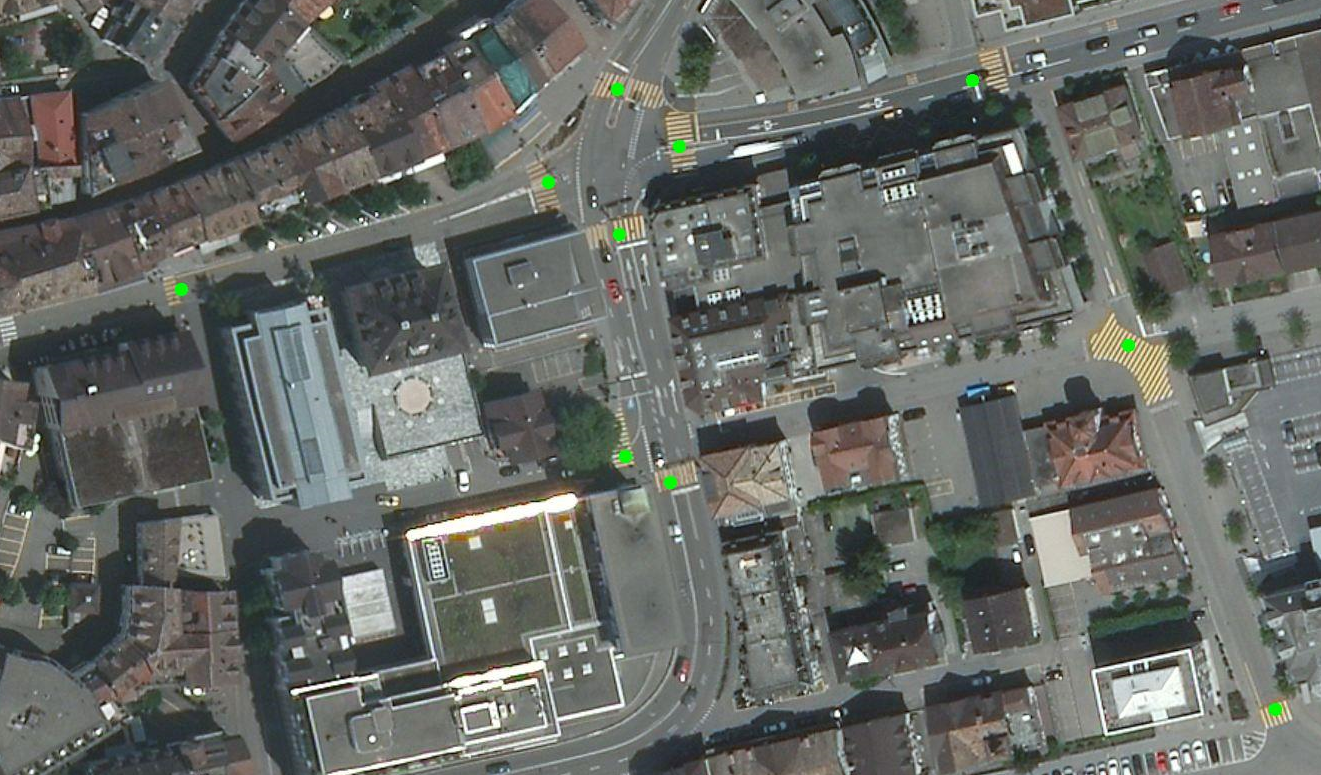
\includegraphics[width=\textwidth -10mm]{images/boxsave_rappi.png}
	\caption[Überblick]{Rapperswil Innenstadt - Gefundene Fussgängerstreifen sind mit einem grünen Punkt markiert.}
\end{figure}
\subsection*{Ausblick}
Der Erkennungsalgorithmus ist zu Ende dieses Projektes auf die Region Zürich und Ostschweiz spezialisiert. Mit weiteren Optimierungen ist es möglich, alle Zebrastreifen in der Schweiz zu erfassen und sogar weisse Zebrastreifen für andere europäische Länder zu erkennen. Auch weitere Strassenmarkierungen sind denkbar.
\newpage